\section{Experimental Evaluation}\label{Se:evaluation}

In this section, we describe quantiative results and share qualitative insight from our evaluation of \Tool. 

\subsection{Experimental Setup and Methodology}

For our experiments, we assembled a suite of 80 Android apps: 4 enterprise apps, 3 apps shipping with version 4.4 of the Android platform, as well as the 73 top-popular Google Play apps in the geography of one of the authors.
The experiments were conducted on a LG Nexus 5 device running version 4.4 of the Android platform (CyanogenMod 11). For accuracy and reproducibility, we reset the device to a clean image before testing each of the apps.

Prior to running \Tool, an independent professional ethical hacker audited all 80 apps. The manual audit consisted in running, and validating by hand the results of, a brute-force fuzzing tool. The tool (i) establishes a crude attack surface by targeting, beyond the {\tt uri} field, all constant strings in the Dalvik bytecode as candidate extra parameters, and (ii) discharges a large amount of pre-defined payloads at each target.

The fuzzing process demanded several hours (if not more) per application, and was carried out over a period of three weeks with multiple instances of the tool running in parallel. It resulted in a total of 163 IAC vulnerabilities. \tableref{vulns} provides a breakdown of the results by issue type.

\subsection{Performance Results}

We have conducted a series of experiments to measure, and thereby justify, the key features of \Tool. We organize our description of the experiments around four research hypotheses. The starting point is a baseline algorithm that only targets declared input points via the {\tt data} field.

\cheapar{H1: Probing Boosts Performance} To quantify the performance gain thanks to probing, we enhanced the baseline algorithm with necessary-conditions specifications as described in \secref{detectionSubsec}. Instead of blindly attempting all possible test payloads, the enhanced version first analyzes the probing trace to focus testing only on relevant attack types.

The statistics demonstrate significant improvement. While naive fuzzing expends an average of 64 tests and 24 minutes per app, the enhanced version requires $<15$ tests and $<7$ minutes per app to detect the same set of IAC vulnerabilities.

\cheapar{H2: String Extras are Often Vulnerable} The naive testing algorithm, equipped with probing capabilities, is able to detect a total of 94 out of the 163 known vulnerabilities for a recall rate of $0.57$. Enhancing it to incorporate string extras as attack targets pushes recall up to 0.85, as 46 new vulnerabilities are detected.

The resulting variant features an iterative testing loop, which attacks targets discovered in previous probing/testing rounds. Naturally, this renders it more expensive than its naive counterpart with an average of 26 (compared to 15) tests and 12 (compared to 7) minutes per app.

\cheapar{H3: Boolean Extras Manifest in Path Conditions} The algorithm featuring both probing and manipulation of string extras already detects 140 out of the 163 known vulnerabilities. A natural means to further increase coverage is by exploring new execution paths.

Augmenting the testing algorithm to explore different combinations of boolean extras achieves this goal effectively. This is seen through the discovery of 11 new vulnerabilities, constituting a 7\% improvement in recall, for a total of 151 vulnerabilities detected fully automatically. 

The cost, as expected, is noticeable. The average number of tests per app climbs by x2.42 from 26 to 63 with a proportional rise of x2.1 in testing time from 12 to 25 minutes. This motivates more efficient detection of new paths.

\cheapar{H4: Linear-time Path Exploration is Effective} The fourth and final hypothesis concerns the relationship between boolean extras in their capacity as branching expressions. The claim is that it is effective to treat boolean extras as either dominating each other or being independent.

Under this assumption, which enables toggling of boolean extras one at a time and thus linear-complexity path exploration, testing time drops to 19 minutes (24\% improvement) and the average number of tests is only 40 compared to 63 before (37\% improvement). At the same time, only one of the 151 vulnerabilities detected via the exponential-time path-exploration algorithm is missed for a negligible drop of $<1$\% in recall.

\cheapar{Discussion} In conclusion, \Tool\ effectively balances performance against coverage.\footnote{
	Beyond the data we present here, which confirms our design choices one atop the other, we have a full matrix of measurements per every combination of the choices we've made. We have omitted most of these measurements for lack of space, but note that they are in strong support of our hypotheses.
} Regarding false negatives, our analysis of the 14 misses (w.r.t. the most comprehensive \Tool\ configuration) reveals that these are caused by one or both of the following reasons: (i) incomplete path coverage (and in particular, path conditions other than boolean extras) and (ii) overly conservative probing checks (where the probe is nontrivially mutated by the app, yet it is possible to craft a successful test payload).

A visual illustration of the performance/coverage tradeoffs achieved by the different variants is provided in \figref{trends}, where \Tool\ is labeled ``Linear PC''.
%
``String Extras'' stands out as the variant that maximizes the recall/performance gap. Even though performance increase exceeds gain in coverage when switching to ``Linear PC'', we still view this option as preferable, as less true warnings are missed in return for affordable performance slowdown.

\begin{figure}
	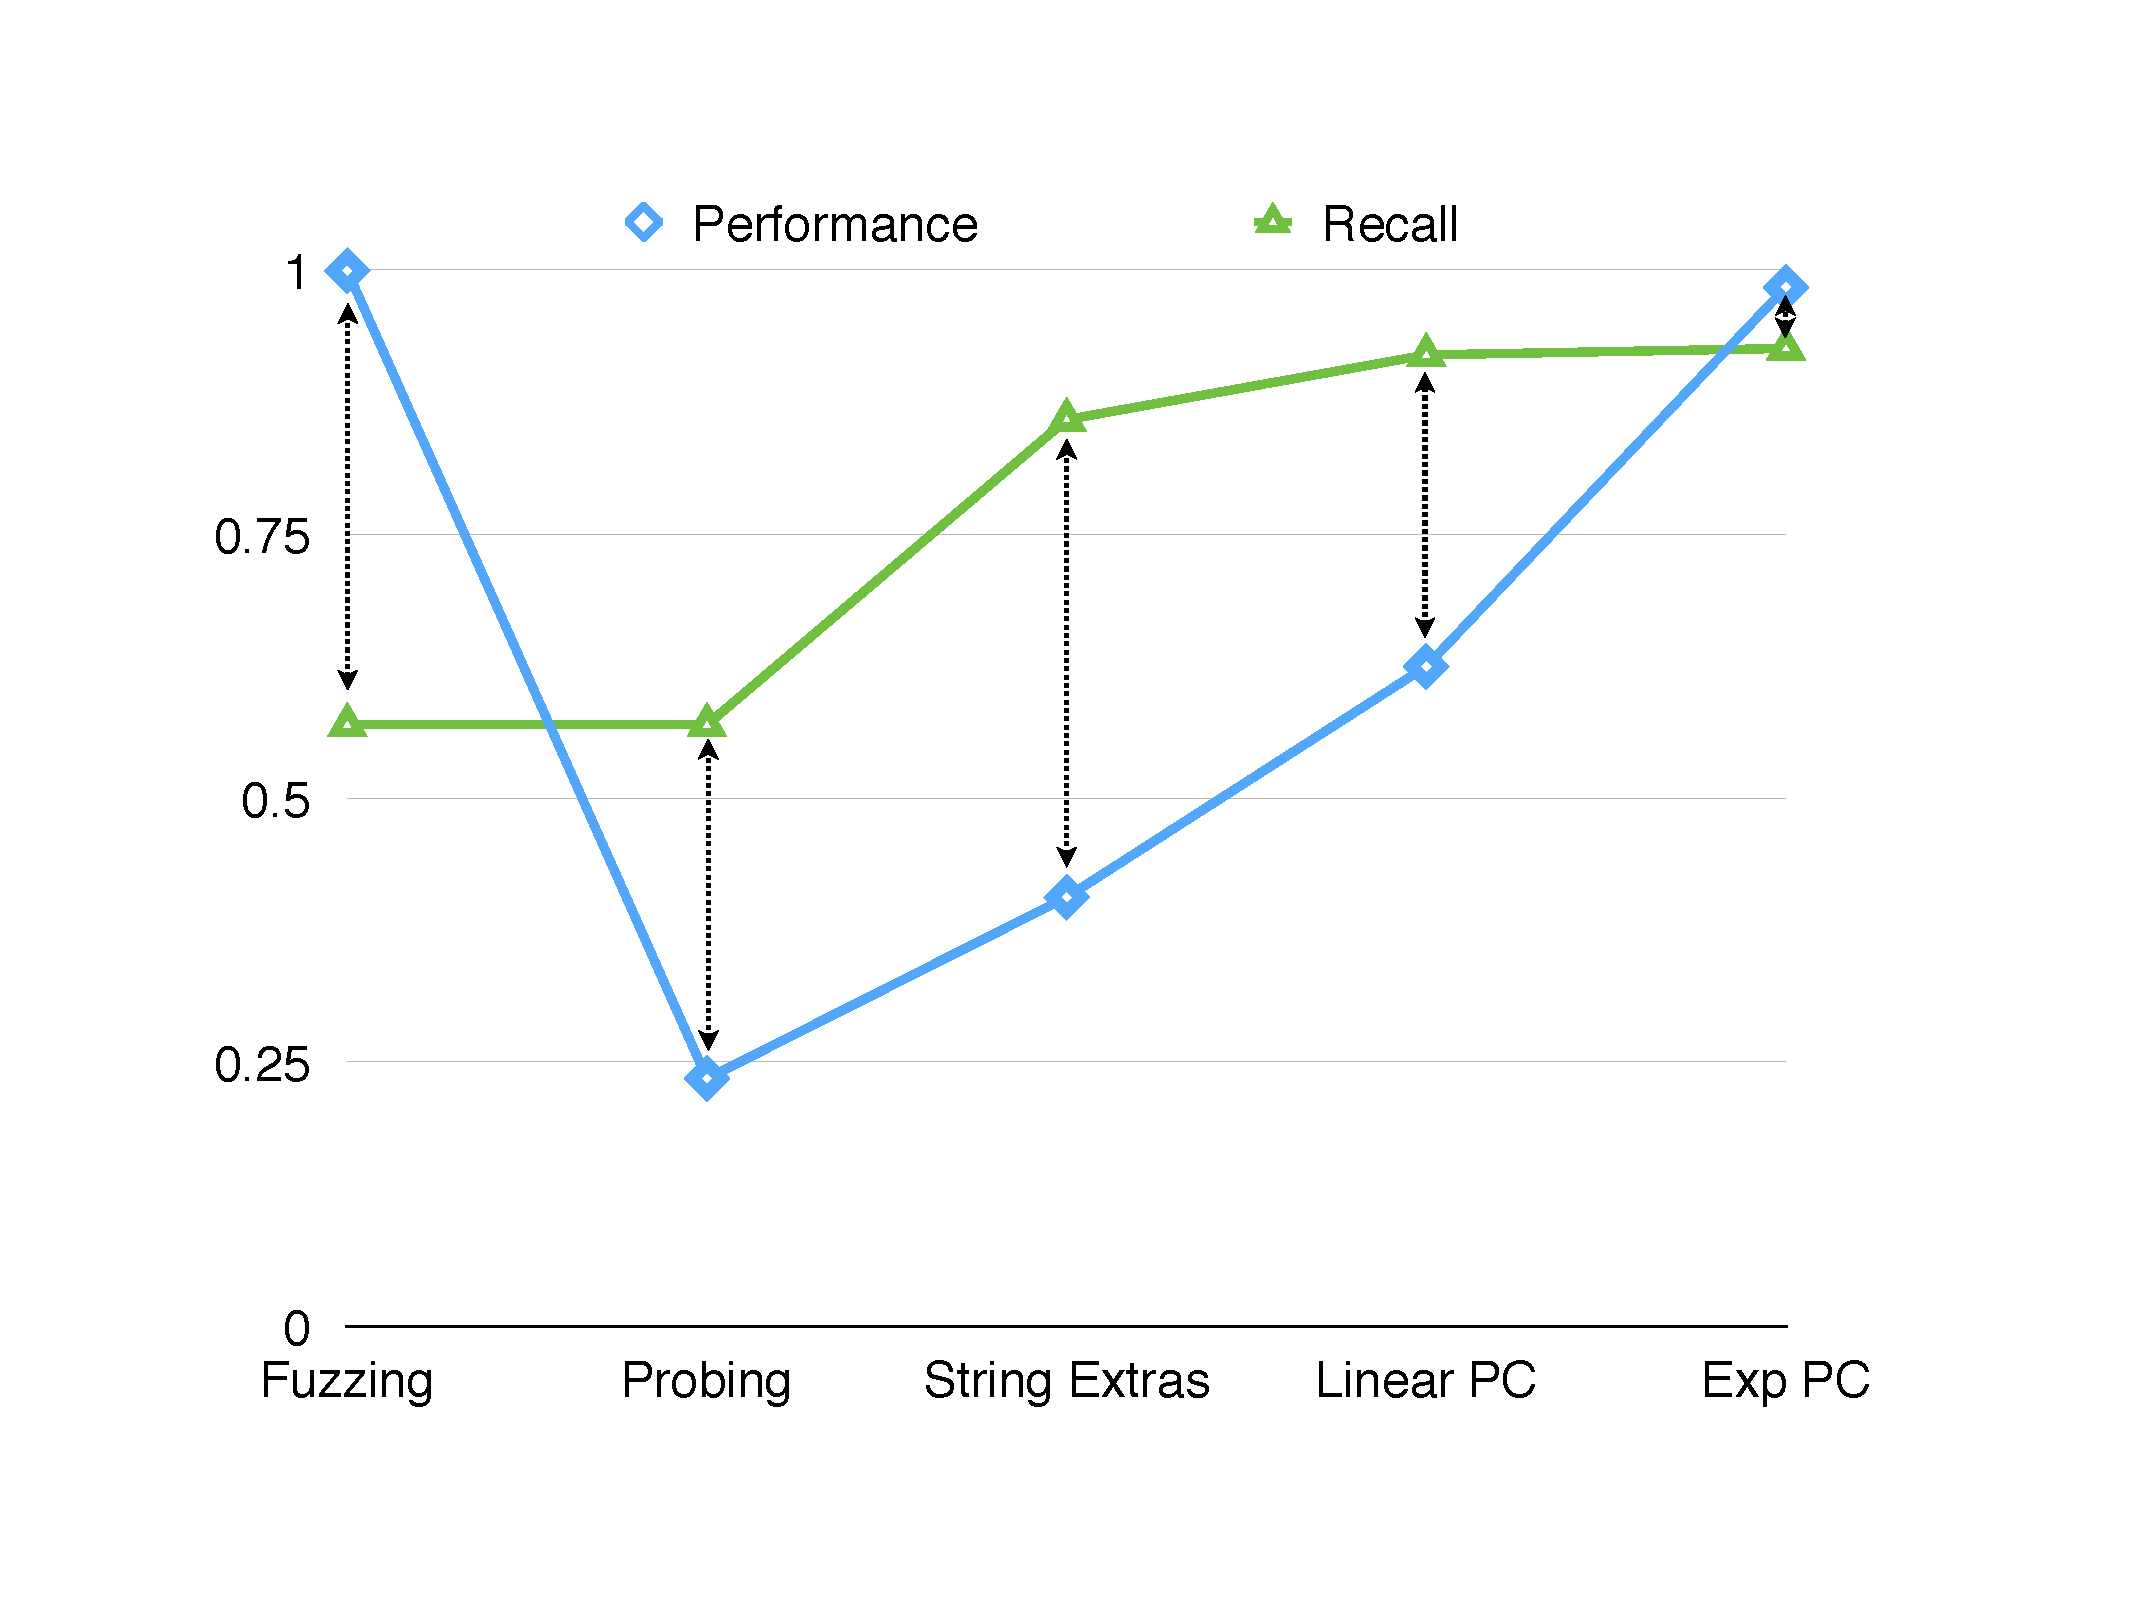
\includegraphics[width=\columnwidth]{trendline.pdf}
	\caption{\label{Fi:trends}Visual Performance/Recall Comparison between Testing Variants}
\end{figure}


\begin{table*}
\def\arraystretch{0.75}
\caption{\label{Ta:vulns}Detected Vulnerabilities with Breakdown by Attack Type}
\begin{scriptsize}
\begin{center}
\begin{tabular}{l|c|c|c|c|c|c|c|c|c|c}
\multicolumn{1}{c|}{\multirow{2}{*}{App Name}} & \multirow{2}{*}{Version} & \multirow{2}{*}{Count} & \multirow{2}{*}{XAS} & \multirow{2}{*}{SQLi} & Unsafe  & UI  & {\tt Fragment}  & Java  & Native  & File  \\
 &  & & &  &  Refl. &  Spoof. &  Injection &  Crash &  Crash &  Man. \\
\hline
com.dropbox.android & 230800 & 4 & \xmark & \xmark & \xmark & \xmark & \cmark & \cmark & \xmark & \xmark \\
com.ebay.mobile & 43 & 3 & \xmark & \xmark & \cmark & \xmark & \xmark & \cmark & \xmark & \xmark \\
com.evernote & 15120 & 7 & \xmark & \xmark & \xmark & \xmark & \cmark & \cmark & \xmark & \xmark \\
com.facebook.katana & 228325 & 4 & \xmark & \xmark & \xmark & \xmark & \xmark & \cmark & \xmark & \xmark \\
com.google.android.gm & 974 & 2 & \xmark & \xmark & \xmark & \xmark & \cmark & \cmark & \xmark & \xmark \\
com.lotus.sync.traveler & 2013062023 & 1 & \xmark & \xmark & \xmark & \xmark & \xmark & \cmark & \xmark & \xmark \\
com.linkedin.android & 56 & 6 & \xmark & \xmark & \xmark & \xmark & \xmark & \cmark & \xmark & \xmark \\
com.nytimes.android & 5523 & 2 & \cmark & \xmark & \xmark & \xmark & \xmark & \cmark & \xmark & \xmark \\
com.google.android.youtube & 4517 & 2 & \xmark & \xmark & \xmark & \xmark & \xmark & \cmark & \xmark & \xmark \\
com.adobe.air & 3700209 & 0 & \xmark & \xmark & \xmark & \xmark & \xmark & \xmark & \xmark & \xmark \\
com.adobe.psmobile & 10 & 0 & \xmark & \xmark & \xmark & \xmark & \xmark & \xmark & \xmark & \xmark \\
com.adobe.reader & 77016 & 3 & \xmark & \xmark & \xmark & \xmark & \xmark & \cmark & \xmark & \xmark \\
com.antivirus & 180265 & 0 & \xmark & \xmark & \xmark & \xmark & \xmark & \xmark & \xmark & \xmark \\
com.android.chrome & 1453090 & 1 & \xmark & \xmark & \xmark & \xmark & \xmark & \cmark & \xmark & \xmark \\
clalit.android & 12 & 0 & \xmark & \xmark & \xmark & \xmark & \xmark & \xmark & \xmark & \xmark \\
com.alibaba.aliexpresshd & 56 & 1 & \xmark & \xmark & \xmark & \xmark & \xmark & \cmark & \xmark & \xmark \\
com.android.vending & 80280020 & 3 & \xmark & \xmark & \xmark & \xmark & \cmark & \cmark & \xmark & \xmark \\
com.box.android & 30200 & 1 & \xmark & \xmark & \xmark & \xmark & \xmark & \cmark & \xmark & \xmark \\
com.cleanmaster.security & 10400566 & 0 & \xmark & \xmark & \xmark & \xmark & \xmark & \xmark & \xmark & \xmark \\
com.fibi & 8 & 0 & \xmark & \xmark & \xmark & \xmark & \xmark & \xmark & \xmark & \xmark \\
com.fitbit.FitbitMobile & 1772 & 1 & \xmark & \xmark & \xmark & \xmark & \xmark & \cmark & \xmark & \xmark \\
com.fitnesskeeper.runkeeper.pro & 215 & 0 & \xmark & \xmark & \xmark & \xmark & \xmark & \xmark & \xmark & \xmark \\
com.google.android.apps.docs.editors.sheets & 1314426 & 4 & \xmark & \xmark & \xmark & \xmark & \xmark & \cmark & \xmark & \xmark \\
com.google.android.apps.m4b & 62 & 0 & \xmark & \xmark & \xmark & \xmark & \xmark & \xmark & \xmark & \xmark \\
com.google.android.apps.magazines & 2014051213 & 0 & \xmark & \xmark & \xmark & \xmark & \xmark & \xmark & \xmark & \xmark \\
com.google.android.apps.maps & 800001324 & 2 & \xmark & \xmark & \xmark & \xmark & \xmark & \cmark & \xmark & \xmark \\
com.google.android.apps.plus & 413004558 & 10 & \xmark & \xmark & \xmark & \xmark & \cmark & \cmark & \cmark & \xmark \\
com.google.android.GoogleCamera & 22024130 & 0 & \xmark & \xmark & \xmark & \xmark & \xmark & \xmark & \xmark & \xmark \\
com.google.android.maps.mytracks & 74 & 3 & \xmark & \xmark & \xmark & \cmark & \xmark & \cmark & \xmark & \xmark \\
com.google.android.music & 1514 & 4 & \xmark & \xmark & \xmark & \xmark & \xmark & \cmark & \xmark & \xmark \\
com.google.android.talk & 21224130 & 1 & \xmark & \cmark & \xmark & \xmark & \xmark & \xmark & \xmark & \xmark \\
com.google.earth & 13294050 & 1 & \xmark & \xmark & \xmark & \xmark & \xmark & \cmark & \xmark & \xmark \\
com.hipmunk.android & 102 & 0 & \xmark & \xmark & \xmark & \xmark & \xmark & \xmark & \xmark & \xmark \\
com.ideomobile.hapoalim & 117 & 12 & \cmark & \xmark & \xmark & \cmark & \xmark & \cmark & \xmark & \xmark \\
com.ideomobile.leumicard & 42 & 2 & \cmark & \xmark & \xmark & \xmark & \xmark & \cmark & \xmark & \xmark \\
com.intsig.camscanner & 3302 & 1 & \xmark & \xmark & \xmark & \xmark & \xmark & \cmark & \xmark & \xmark \\
com.leumi.leumiwallet & 18 & 1 & \xmark & \xmark & \xmark & \xmark & \xmark & \cmark & \xmark & \xmark \\
com.melodis.midomiMusicIdentifier.freemium & 10602 & 2 & \cmark & \xmark & \xmark & \xmark & \xmark & \cmark & \xmark & \xmark \\
com.mxtech.videoplayer.ad & 700000070 & 2 & \xmark & \xmark & \xmark & \xmark & \cmark & \cmark & \xmark & \xmark \\
com.netgate & 141 & 0 & \xmark & \xmark & \xmark & \xmark & \xmark & \xmark & \xmark & \xmark \\
com.nike.plusgps & 99 & 0 & \xmark & \xmark & \xmark & \xmark & \xmark & \xmark & \xmark & \xmark \\
com.onoapps.cal4u & 5 & 0 & \xmark & \xmark & \xmark & \xmark & \xmark & \xmark & \xmark & \xmark \\
com.paypal.android.p2pmobile & 49 & 1 & \xmark & \xmark & \xmark & \xmark & \xmark & \cmark & \xmark & \xmark \\
com.runtastic.android & 90 & 1 & \xmark & \xmark & \xmark & \xmark & \xmark & \cmark & \xmark & \xmark \\
com.snapchat.android & 323 & 0 & \xmark & \xmark & \xmark & \xmark & \xmark & \xmark & \xmark & \xmark \\
com.ubercab & 30618 & 0 & \xmark & \xmark & \xmark & \xmark & \xmark & \xmark & \xmark & \xmark \\
com.urbandroid.sleep & 842 & 4 & \xmark & \xmark & \xmark & \xmark & \cmark & \cmark & \xmark & \xmark \\
com.viber.voip & 61 & 2 & \xmark & \xmark & \xmark & \xmark & \xmark & \cmark & \xmark & \xmark \\
com.waze & 1019718 & 1 & \xmark & \xmark & \xmark & \xmark & \xmark & \cmark & \xmark & \xmark \\
com.yahoo.mobile.client.android.flickr & 41700 & 0 & \xmark & \xmark & \xmark & \xmark & \xmark & \xmark & \xmark & \xmark \\
com.yelp.android & 10000903 & 4 & \xmark & \xmark & \xmark & \xmark & \xmark & \cmark & \xmark & \xmark \\
com.android.contacts & 19 & 7 & \xmark & \xmark & \xmark & \cmark & \xmark & \cmark & \xmark & \xmark \\
com.android.dialer & 19 & 2 & \xmark & \xmark & \xmark & \xmark & \xmark & \cmark & \xmark & \xmark \\
com.facebook.orca & 221196 & 1 & \xmark & \xmark & \cmark & \xmark & \xmark & \xmark & \xmark & \xmark \\
com.facebook.pages.app & 232657 & 1 & \xmark & \xmark & \cmark & \xmark & \xmark & \xmark & \xmark & \xmark \\
org.mozilla.firefox & 2013061803 & 6 & \xmark & \xmark & \xmark & \cmark & \xmark & \cmark & \xmark & \cmark \\
com.gau.go.launcherex & 234 & 2 & \xmark & \xmark & \xmark & \xmark & \xmark & \cmark & \xmark & \xmark \\
com.google.android.apps.currents & 130781200 & 0 & \xmark & \xmark & \xmark & \xmark & \xmark & \xmark & \xmark & \xmark \\
com.google.android.apps.docs & 1218226 & 5 & \xmark & \xmark & \xmark & \cmark & \xmark & \cmark & \xmark & \xmark \\
com.google.android.apps.finance & 35 & 2 & \xmark & \xmark & \xmark & \xmark & \xmark & \cmark & \xmark & \xmark \\
com.google.android.apps.translate & 20700177 & 2 & \xmark & \xmark & \cmark & \xmark & \xmark & \cmark & \xmark & \xmark \\
org.dayup.gtask & 1602 & 11 & \xmark & \xmark & \xmark & \xmark & \cmark & \cmark & \xmark & \xmark \\
com.ibm.lotus.connections.mobile & 2013092105 & 5 & \xmark & \xmark & \xmark & \xmark & \xmark & \cmark & \xmark & \xmark \\
com.ibm.android.sametime.meetings & 20130528 & 3 & \xmark & \xmark & \xmark & \xmark & \xmark & \cmark & \xmark & \xmark \\
com.ibm.android.sametime & 2013041715 & 1 & \xmark & \xmark & \xmark & \xmark & \xmark & \cmark & \xmark & \xmark \\
com.ibm.mobile.android.unyte & 20121206 & 0 & \xmark & \xmark & \xmark & \xmark & \xmark & \xmark & \xmark & \xmark \\
com.imdb.mobile & 103220310 & 0 & \xmark & \xmark & \xmark & \xmark & \xmark & \xmark & \xmark & \xmark \\
com.instagram.android & 197069 & 3 & \xmark & \xmark & \xmark & \xmark & \xmark & \cmark & \xmark & \xmark \\
com.android.mms & 19 & 3 & \xmark & \xmark & \xmark & \cmark & \xmark & \cmark & \xmark & \xmark \\
mobi.mgeek.TunnyBrowser & 331 & 1 & \xmark & \xmark & \xmark & \xmark & \xmark & \cmark & \xmark & \xmark \\
com.opera.browser.beta & 1600559192 & 0 & \xmark & \xmark & \xmark & \xmark & \xmark & \xmark & \xmark & \xmark \\
org.telegram.messenger & 227 & 0 & \xmark & \xmark & \xmark & \xmark & \xmark & \xmark & \xmark & \xmark \\
org.zwanoo.android.speedtest & 124 & 1 & \xmark & \xmark & \xmark & \xmark & \xmark & \cmark & \xmark & \xmark \\
com.shazam.android & 78059 & 5 & \cmark & \xmark & \xmark & \xmark & \xmark & \cmark & \xmark & \xmark \\
com.skype.raider & 50469393 & 0 & \xmark & \xmark & \xmark & \xmark & \xmark & \xmark & \xmark & \xmark \\
com.sgiggle.production & 53 & 3 & \xmark & \xmark & \xmark & \xmark & \xmark & \cmark & \xmark & \xmark \\
com.ted.android & 18 & 0 & \xmark & \xmark & \xmark & \xmark & \xmark & \xmark & \xmark & \xmark \\
com.devuni.flashlight & 139 & 0 & \xmark & \xmark & \xmark & \xmark & \xmark & \xmark & \xmark & \xmark \\
com.whatsapp & 47672 & 0 & \xmark & \xmark & \xmark & \xmark & \xmark & \xmark & \xmark & \xmark \\
fr.beungoud.xbmcremote & 47 & 0 & \xmark & \xmark & \xmark & \xmark & \xmark & \xmark & \xmark & \xmark \\ 
\hline\hline
\multicolumn{1}{c|}{{\bf 55/80}} & & {\bf 163} & {\bf 5} & {\bf 1} & {\bf 4}  & {\bf 6}  & {\bf 8} & {\bf 30} & {\bf 1} & {\bf 1} \\
%\_Dropbox v2.3.8 & 4 & \xmark & \xmark & \xmark & \xmark & \cmark & \cmark & \xmark & \xmark \\
%\_eBay v2.3.0.25 & 3 & \xmark & \xmark & \cmark & \xmark & \xmark & \cmark & \xmark & \xmark \\
%\_Evernote v5.1.2 & 7 & \xmark & \xmark & \xmark & \xmark & \cmark & \cmark & \xmark & \xmark \\
%\_Facebook v3.3 & 4 & \xmark & \xmark & \xmark & \xmark & \xmark & \cmark & \xmark & \xmark \\
%\_Gmail v4.5-836823 & 2 & \xmark & \xmark & \xmark & \xmark & \cmark & \cmark & \xmark & \xmark \\
%\_IBM Notes Traveler v9.0.0.0 201306202317 & 1 & \xmark & \xmark & \xmark & \xmark & \xmark & \cmark & \xmark & \xmark \\
%\_LinkedIn v3.0.2 & 6 & \xmark & \xmark & \xmark & \xmark & \xmark & \cmark & \xmark & \xmark \\
%\_NYTimes for Android v3.2.2 & 2 & \cmark & \xmark & \xmark & \xmark & \xmark & \cmark & \xmark & \xmark \\
%\_YouTube v4.5.17 & 2 & \xmark & \xmark & \xmark & \xmark & \xmark & \cmark & \xmark & \xmark \\
%Adobe AIR v3.7.0.209 & 0 & \xmark & \xmark & \xmark & \xmark & \xmark & \xmark & \xmark & \xmark \\
%Adobe Photoshop Express v1.3.3 & 0 & \xmark & \xmark & \xmark & \xmark & \xmark & \xmark & \xmark & \xmark \\
%Adobe Reader v10.6.0 & 3 & \xmark & \xmark & \xmark & \xmark & \xmark & \cmark & \xmark & \xmark \\
%Antivirus Security - FREE v3.2.3 & 0 & \xmark & \xmark & \xmark & \xmark & \xmark & \xmark & \xmark & \xmark \\
%Chrome Browser - Google v27.0.1453.90 & 1 & \xmark & \xmark & \xmark & \xmark & \xmark & \cmark & \xmark & \xmark \\
%clalit.android-1. & 0 & \xmark & \xmark & \xmark & \xmark & \xmark & \xmark & \xmark & \xmark \\
%com.alibaba.aliexpresshd-1. & 1 & \xmark & \xmark & \xmark & \xmark & \xmark & \cmark & \xmark & \xmark \\
%com.android.vending-1 & 3 & \xmark & \xmark & \xmark & \xmark & \cmark & \cmark & \xmark & \xmark \\
%com.box.android-1. & 1 & \xmark & \xmark & \xmark & \xmark & \xmark & \cmark & \xmark & \xmark \\
%com.cleanmaster.security-1. & 0 & \xmark & \xmark & \xmark & \xmark & \xmark & \xmark & \xmark & \xmark \\
%com.fibi-1 & 0 & \xmark & \xmark & \xmark & \xmark & \xmark & \xmark & \xmark & \xmark \\
%com.fitbit.FitbitMobile-1. & 1 & \xmark & \xmark & \xmark & \xmark & \xmark & \cmark & \xmark & \xmark \\
%com.fitnesskeeper.runkeeper.pro-1. & 0 & \xmark & \xmark & \xmark & \xmark & \xmark & \xmark & \xmark & \xmark \\
%com.google.android.apps.docs.editors.sheets-1. & 4 & \xmark & \xmark & \xmark & \xmark & \xmark & \cmark & \xmark & \xmark \\
%com.google.android.apps.m4b-1. & 0 & \xmark & \xmark & \xmark & \xmark & \xmark & \xmark & \xmark & \xmark \\
%com.google.android.apps.magazines-1. & 0 & \xmark & \xmark & \xmark & \xmark & \xmark & \xmark & \xmark & \xmark \\
%com.google.android.apps.maps-1. & 2 & \xmark & \xmark & \xmark & \xmark & \xmark & \cmark & \xmark & \xmark \\
%com.google.android.apps.plus-1. & 10 & \xmark & \xmark & \xmark & \xmark & \cmark & \cmark & \cmark & \xmark \\
%com.google.android.GoogleCamera-1 & 0 & \xmark & \xmark & \xmark & \xmark & \xmark & \xmark & \xmark & \xmark \\
%com.google.android.maps.mytracks-1. & 3 & \xmark & \xmark & \xmark & \cmark & \xmark & \cmark & \xmark & \xmark \\
%com.google.android.music-1. & 4 & \xmark & \xmark & \xmark & \xmark & \xmark & \cmark & \xmark & \xmark \\
%com.google.android.talk-2. & 1 & \xmark & \cmark & \xmark & \xmark & \xmark & \xmark & \xmark & \xmark \\
%com.google.earth-1. & 1 & \xmark & \xmark & \xmark & \xmark & \xmark & \cmark & \xmark & \xmark \\
%com.hipmunk.android-1. & 0 & \xmark & \xmark & \xmark & \xmark & \xmark & \xmark & \xmark & \xmark \\
%com.ideomobile.hapoalim-1. & 12 & \cmark & \xmark & \xmark & \cmark & \xmark & \cmark & \xmark & \xmark \\
%com.ideomobile.leumicard-1 & 2 & \cmark & \xmark & \xmark & \xmark & \xmark & \cmark & \xmark & \xmark \\
%com.intsig.camscanner-1. & 1 & \xmark & \xmark & \xmark & \xmark & \xmark & \cmark & \xmark & \xmark \\
%com.leumi.leumiwallet-1. & 1 & \xmark & \xmark & \xmark & \xmark & \xmark & \cmark & \xmark & \xmark \\
%com.melodis.midomiMusicIdentifier.freemium-1. & 2 & \cmark & \xmark & \xmark & \xmark & \xmark & \cmark & \xmark & \xmark \\
%com.mxtech.videoplayer.ad-1. & 2 & \xmark & \xmark & \xmark & \xmark & \cmark & \cmark & \xmark & \xmark \\
%com.netgate-1 & 0 & \xmark & \xmark & \xmark & \xmark & \xmark & \xmark & \xmark & \xmark \\
%com.nike.plusgps-1. & 0 & \xmark & \xmark & \xmark & \xmark & \xmark & \xmark & \xmark & \xmark \\
%com.onoapps.cal4u-1 & 0 & \xmark & \xmark & \xmark & \xmark & \xmark & \xmark & \xmark & \xmark \\
%com.paypal.android.p2pmobile-1 & 1 & \xmark & \xmark & \xmark & \xmark & \xmark & \cmark & \xmark & \xmark \\
%com.runtastic.android-1. & 1 & \xmark & \xmark & \xmark & \xmark & \xmark & \cmark & \xmark & \xmark \\
%com.snapchat.android-1. & 0 & \xmark & \xmark & \xmark & \xmark & \xmark & \xmark & \xmark & \xmark \\
%com.ubercab-1. & 0 & \xmark & \xmark & \xmark & \xmark & \xmark & \xmark & \xmark & \xmark \\
%com.urbandroid.sleep-1. & 4 & \xmark & \xmark & \xmark & \xmark & \cmark & \cmark & \xmark & \xmark \\
%com.viber.voip-1. & 2 & \xmark & \xmark & \xmark & \xmark & \xmark & \cmark & \xmark & \xmark \\
%com.waze-1. & 1 & \xmark & \xmark & \xmark & \xmark & \xmark & \cmark & \xmark & \xmark \\
%com.yahoo.mobile.client.android.flickr-1. & 0 & \xmark & \xmark & \xmark & \xmark & \xmark & \xmark & \xmark & \xmark \\
%com.yelp.android-1. & 4 & \xmark & \xmark & \xmark & \xmark & \xmark & \cmark & \xmark & \xmark \\
%Contacts. & 7 & \xmark & \xmark & \xmark & \cmark & \xmark & \cmark & \xmark & \xmark \\
%Dialer. & 2 & \xmark & \xmark & \xmark & \xmark & \xmark & \cmark & \xmark & \xmark \\
%Facebook Messenger v2.5.3-release & 1 & \xmark & \xmark & \cmark & \xmark & \xmark & \xmark & \xmark & \xmark \\
%Facebook Pages Manager v1.4.1 & 1 & \xmark & \xmark & \cmark & \xmark & \xmark & \xmark & \xmark & \xmark \\
%Firefox Browser for Android v22.0 & 6 & \xmark & \xmark & \xmark & \cmark & \xmark & \cmark & \xmark & \cmark \\
%GO Launcher EX v3.9.11 & 2 & \xmark & \xmark & \xmark & \xmark & \xmark & \cmark & \xmark & \xmark \\
%Google Currents v2.1.0 & 0 & \xmark & \xmark & \xmark & \xmark & \xmark & \xmark & \xmark & \xmark \\
%Google Drive v1.2.182.26 & 5 & \xmark & \xmark & \xmark & \cmark & \xmark & \cmark & \xmark & \xmark \\
%Google Finance v2.2.7 & 2 & \xmark & \xmark & \xmark & \xmark & \xmark & \cmark & \xmark & \xmark \\
%Google Translate v2.7 & 2 & \xmark & \xmark & \cmark & \xmark & \xmark & \cmark & \xmark & \xmark \\
%GTasks v1.6.0.2 & 11 & \xmark & \xmark & \xmark & \xmark & \cmark & \cmark & \xmark & \xmark \\
%IBM Connections v4.4.0 & 5 & \xmark & \xmark & \xmark & \xmark & \xmark & \cmark & \xmark & \xmark \\
%IBM Sametime Meetings v8.5.2.4 & 3 & \xmark & \xmark & \xmark & \xmark & \xmark & \cmark & \xmark & \xmark \\
%IBM Sametime v8.5.2.4 201304171550 & 1 & \xmark & \xmark & \xmark & \xmark & \xmark & \cmark & \xmark & \xmark \\
%IBM SmartCloud Meetings v8.5.2.1.201212060646 & 0 & \xmark & \xmark & \xmark & \xmark & \xmark & \xmark & \xmark & \xmark \\
%IMDB Movies And TV v3.2.2.103220310 & 0 & \xmark & \xmark & \xmark & \xmark & \xmark & \xmark & \xmark & \xmark \\
%Instagram v3.5.3 & 3 & \xmark & \xmark & \xmark & \xmark & \xmark & \cmark & \xmark & \xmark \\
%Mms & 3 & \xmark & \xmark & \xmark & \cmark & \xmark & \cmark & \xmark & \xmark \\
%mobi.mgeek.TunnyBrowser-1. & 1 & \xmark & \xmark & \xmark & \xmark & \xmark & \cmark & \xmark & \xmark \\
%Opera browser beta v15.0.1162.59192 & 0 & \xmark & \xmark & \xmark & \xmark & \xmark & \xmark & \xmark & \xmark \\
%org.telegram.messenger-1. & 0 & \xmark & \xmark & \xmark & \xmark & \xmark & \xmark & \xmark & \xmark \\
%org.zwanoo.android.speedtest-1 & 1 & \xmark & \xmark & \xmark & \xmark & \xmark & \cmark & \xmark & \xmark \\
%Shazam v3.14.0-JB78059 & 5 & \cmark & \xmark & \xmark & \xmark & \xmark & \cmark & \xmark & \xmark \\
%Skype - free IM and video calls v3.2.0.6673 & 0 & \xmark & \xmark & \xmark & \xmark & \xmark & \xmark & \xmark & \xmark \\
%Tango Text Voice and Video v2.10.48610 & 3 & \xmark & \xmark & \xmark & \xmark & \xmark & \cmark & \xmark & \xmark \\
%TED v1.1.6 & 0 & \xmark & \xmark & \xmark & \xmark & \xmark & \xmark & \xmark & \xmark \\
%Tiny Flashlight + LED v4.9.4 & 0 & \xmark & \xmark & \xmark & \xmark & \xmark & \xmark & \xmark & \xmark \\
%WhatsApp Messenger v2.10.222 & 0 & \xmark & \xmark & \xmark & \xmark & \xmark & \xmark & \xmark & \xmark \\
%XBMC remote control v2.0.1 & 0 & \xmark & \xmark & \xmark & \xmark & \xmark & \xmark & \xmark & \xmark \\ 
%\hline\hline
%\multicolumn{1}{c|}{{\bf 55/80}} & {\bf 163} & {\bf 5} & {\bf 1} & {\bf 4}  & {\bf 6}  & {\bf 8} & {\bf 30} & {\bf 1} & {\bf 1} \\
\end{tabular}
\end{center}
\end{scriptsize}
\end{table*}

\subsection{Interesting Vulnerabilities}\label{Se:caseStudies}

Though all vulnerabilities specified above are exploitable, most of them are of 
low severity as they either only impact the stability of the target app or assume a complex payload/vector that is hard to create in practice.
%
Other findings are of high severity, as they impact the confidentiality of user data, the integrity of the application or both, and we were able to demonstrate a concrete exploit for them. We conclude by
highlighting three of these vulnerabilities. We have reported these vulnerabilities to the developers. In all cases, the vulnerable scenario was confirmed as such and was fixed shortly thereafter.

\cheapar{Preference Activities and Fragment Loading}\label{Se:PreferenceActivities}
The Android framework provides an abstract {\tt Activity} class,\texttt{
android.preference.PreferenceActivity}, which serves as a reusable and extensible preferences dialog. 
The {\tt PreferenceActivity} class queries its input {\tt Intent} for several extra data fields. These include fields \texttt{EXTRA\_SHOW\_FRAGMENT}
(\texttt{show\_fragment}) 
as well as \texttt{EXTRA\_SHOW\_FRAGMENT\_ARGUMENTS}.
(\texttt{show\_fragment\_arguments}).

The first of these fields specifies the name 
of a \texttt{Fragment} class, which \texttt{PreferenceActivity}
displays dynamically upon being created. The {\tt Fragment.Instantiate($\ldots$)} method creates a {\tt Fragment} instance dynamically, via reflection, and then
casts it into the {\tt Fragment} type.

The second field is the \texttt{Fragment}'s input {\tt Bundle}. A loaded \texttt{Fragment} can
receive input arguments by accessing its host activity (and therefore
its input \texttt{Intent}) using the \texttt{Fragment.getActivity()} API. The second field therefore provides the additional arguments required to instantiate the {\tt Fragment} (if any).

Any app containing an exported {\tt Activity} that extends the {\tt PreferenceActivity} class can be subverted to load an arbitrary class (available to the class loader of the target application)
by exploiting the unsafe dynamic {\tt Fragment} loading process. \Tool\ was indeed able to take advantage of this weakness
in several applications --- including Gmail, Google Translate and Dropbox --- by
targeting the \texttt{show\_fragment}  field with {\tt Fragment} class names from the Android framework and providing corresponding arguments via the \texttt{show\_fragment\_arguments} field. 

%These were loaded successfully, since
%the class loader assigned to the context of \texttt{PreferenceActivity} is the core
%\texttt{PathClassLoader}, which can load any class from the app itself as well as the Android and Java libraries.

As a notable example, \Tool\ was able to inject integrity payloads via the input {\tt Bundle} in Android's built-in Settings app, where {\tt PreferenceActivity} is used. 
The vulnerability detected by \Tool\ allows a malicious app to load an instance of \texttt{ChooseLockPasswordFragment}
and feed data into it despite its normal instantiation under a non-exported
activity. A user can then bypass insertion of the old PIN number when changing PINs by setting the \texttt{confirm\_credentials} field to \texttt{false}.

%\begin{figure}
%	\includegraphics[width=\columnwidth]{CaseStudy1.pdf}
%	\caption{\label{Fi:caseStudy1}Visual Representation of the Testing Scenario Exposing the {\tt Fragment}-injection Vulnerability in the Settings System App}
%\end{figure}

We have reported this severe issue to the Android security team. In response, they
created a patch for \texttt{PreferenceActivity} starting Android 4.4 KitKat. 
The patched class contains a new method, \texttt{isValidFragment(String fragmentName)}, 
where the Android SDK clearly states that 
``\textit{[s]ubclasses should override this method to verify that the given fragment is a valid type to be attached to this activity}''.
%which is documented as follows in the Android SDK:
%\begin{quote}
%	``\textit{Added in API level 19}
%	
%	Subclasses should override this method and verify that the given fragment
%	is a valid type to be attached to this activity. The default implementation
%	returns true for apps built for \texttt{targetSdkVersion}
%	older than \texttt{KITKAT}. For later versions, it will throw an exception.
%	
%	\textit{Parameters} \texttt{fragmentName} the class name of the Fragment
%	about to be attached to this activity. 
%	
%	\textit{Returns} true if the fragment class name is valid for this
%	Activity and false otherwise which is called before the fragment is
%	instantiated.'' 
%\end{quote}
%It is the responsibility of the developer to override method {\tt isValidFragment($\ldots$)} to whitelist the {\tt Fragment}s that are allowed to be loaded within a specific
%{\tt Activity}.

\cheapar{XAS Weakness in Apache Cordova}\label{Se:CordovaXAS}

Apache Cordova is among the most prevalent Android frameworks, serving as the basis of 5.8\% of all Android applications and 1.2\% of the top 500 apps in the Google-Play store.\footnote{\url{http://www.appbrain.com/stats/libraries/details/phonegap/phonegap-apache-cordova}} Cordova exposes a set of APIs that allow the developer to access native device functionality, such as the camera or accelerometer, from JavaScript. Combined with a UI framework like jQuery, Cordova enables the development of smartphone apps based only
on HTML, CSS and JavaScript. This is forming into a strong trend. Indeed as of July 2014, 7.8\% of all new apps (30 days old or younger) are built atop Cordova, which indicates that Cordova is increasingly gaining popularity.

Applications written on top of Cordova make use of a {\tt WebView} instance to interact with the user. When the application is first loaded, it invokes the {\tt loadUrl($\ldots$)} method of the {\tt CordovaWebView} class, which is a subtype of {\tt Activity}. {\tt loadUrl($\ldots$)} has the following implementation:
\begin{small}
\begin{lstlisting}[showstringspaces=false]
public void loadUrl(String url) {
  if (url.equals("about:blank") || 
      url.startsWith("javascript:")) { this.loadUrlNow(url); }
  else {
    String initUrl = this.getProperty("url", null); }
    // If fst page, then set URL to load to be the one passed in
    if (initUrl == null) { this.loadUrlIntoView(url); }
    // Otherwise use the URL specified in the extras bundle
    else { this.loadUrlIntoView(initUrl); } }
\end{lstlisting}
\end{small}
As the code shows, the {\tt initUrl} string is defined as the result of a  {\tt getProperty("url", null)} call, which consists of the following code:
\begin{small}
\begin{lstlisting}[showstringspaces=false]
public String getProperty(String name, String defaultValue) {
  Bundle bdl = cordova.getActivity().getIntent().getExtras();
  if (bdl == null) { return defaultValue; }
  Object p = bdl.get(name);
  if (p == null) { return defaultValue; }
  return p.toString(); }
\end{lstlisting}
\end{small}
The return value of {\tt getProperty($\ldots$)} is an extra parameter obtained from the {\tt Bundle} object associated with the current {\tt Intent} (which, in turn, is retrieved via the {\tt getIntent().getExtras()} getter chain). Thus, variable {\tt url} in {\tt loadUrl($\ldots$)}, flowing into the {\tt loadUrlIntoView} call, opens the opportunity for an attack. This variable is defined
as the value of the {\tt 'url'} extra parameters, which can be set externally.  
Thus, a malicious caller could launch the {\tt Activity} with an {\tt Intent} whose respective {\tt Bundle} maps {\tt 'url'} to an unintended value. The provided URL will consequently be loaded by Cordova and rendered within the {\tt WebView}.

This vulnerability enables theft of sensitive data (such as login credentials) owned by any Cordova-based app having the vulnerable {\tt WebView} embedded in a public {\tt Activity}.
We emphasize that in the described scenario, the {\tt 'url'} extra parameter is fetched directly from the extras {\tt Bundle}. 

\Tool\ was able to successfully detect this nontrivial vulnerability using its ability to track indirect accesses to extra parameters, as described in \secref{customparams}.
We  disclosed this acute issue to the Cordova team as CVE-2014-3500. The Cordova team has issued a patch starting version 3.5.1 of the framework.

\cheapar{File Manipulation in the Firefox Browser}\label{Se:FirefoxFileManipulation}
Public class {\tt org.mozilla.gecko.CrashReporter} extends {\tt Activity}. Its purpose is to send crash dumps to Mozilla when the Firefox browser treminates unexpectedly.
{\tt CrashReporter}, a subclass of {\tt Activity}, receives the dump file path as input via an extra {\tt Intent} parameter called {\tt minidumpPath}. When this {\tt Activity} is launched, its {\tt onCreate($\ldots$)} method is executed, triggering the following sequence of actions:
\begin{compactenum}
	\item Using the \texttt{moveFile($\ldots$)} method, the current dump file is moved to the pending dump-files path: \texttt{files/mozilla/Crash Reports/pending}.
	\item A metadata filename is derived from the given dump file path by replacing all occurrences of the {\tt .dmp} file extension with  {\tt .extra}. 
	\item The metadata file is subsequently moved to the pending dump-files path using the \texttt{moveFile($\ldots$)} method.
	\item The metadata file is parsed into key/value format. The target server's URL (i.e., the URL of the server that the crash information is sent to) is specified there using the \texttt{ServerURL} key.
	\item The {\tt CrashReporter} dialog is displayed to the user.
	\item Finally, when the user presses either the ``Close'' or the ``Restart'' button with the ``Send report'' checkbox enabled, the dump file --- along with other sensitive information --- are sent to the specified server by invoking the {\tt sendReport($\ldots$)} method. Note that if the user further checks the ``Include the address'' checkbox, then Android logs are sent as well.
\end{compactenum}

The security problem created by this scenario traces back to {\tt CrashReporter} and its treatment of the {\tt minidumpPath} extra parameter as trusted, where in fact it should be treated as untrusted, as it is specified by an external agent.
%
Indeed, an adversarial agent can manipulate the source path of the moved file as well as the deduced extra file. 
This manipulation enables control over the server that the crash dump is reported to, in addition to controlling the path of the crash dump file, which allows theft of sensitive information.

We have disclosed this issue as CVE-2014-1506 to the Mozilla security team, which released a fixed version shortly afterwards.\footnote{\url{https://www.mozilla.org/security/announce/2014/mfsa2014-24.html}} 
	\Tool\ was able to detect this issue by discovering the {\tt minidumpPath} extra parameter and recording calls to {\tt File.renameTo($\ldots$)} and {\tt File.createNewFile()}, wherein the initialized {\tt File} object is mapped to  a user-controlled path.